% kapitel2.tex
\chapter{Least Loaded Link First Algorithmus}
\label{chapter:algorithmus1}

Der \textit{Least Loaded Link First} (LLLF) Algorithmus ist ein heuristisches Verfahren zur Pfadwahl in Kommunikationsnetzen. Ziel ist es, Anfragen für Datenübertragungen so durch das Netzwerk zu leiten, dass die Auslastung einzelner Kanten möglichst gleichmäßig verteilt wird (Maximum Link Utilisation MLU). Dadurch sollen Engpässe vermieden und die Gesamteffizienz des Netzwerks gesteigert werden.

\section{Grundidee}
    Im Gegensatz zu klassischen Routingverfahren, die z. B. nur auf minimale Pfadlänge oder Kosten achten, berücksichtigt der LLLF-Ansatz die aktuelle Belastung der Netzwerkressourcen. Jeder Übertragungswunsch (Demand) wird nacheinander betrachtet, und für ihn wird ein Pfad gesucht, der die zukünftige maximale Auslastung des Netzes minimal hält. Dies geschieht durch eine Abwandlung des Dijkstra-Algorithmus, die nicht die Länge der Pfade, sondern die relative Auslastung der Links als Kostenfunktion verwendet. \\
    In Algorithmus \ref{alg:lllf_solver} wurde eine sehr simple Umsetzung in Pseudo-Code erstellt.
    
    \begin{algorithm}[H]
        \caption{LLLF-Solver}
        \label{alg:lllf_solver}
        \begin{algorithmic}[1]
            \Require $G(V,E,c:E\mapsto\mathbb{R})$, $D=\{ D_1=(s_1,t_1,d_1), D_2, \dots, D_n \}$
            \Ensure $P=\{P_1, P_2, \dots, P_n\}$
            \For{$e\in E$} 
                \State $loads_e \gets 0$
            \EndFor
            \State $P \gets \{\}$
            \For{$i \in \{1,\dots,n\}$} 
                \State $P_i \gets PotentialUtilizationDijkstra(G, loads, D_i)$
                \For{$e \in P_i$} 
                    \State $loads_e \gets loads_e + d_i$
                    \State $utilization_e \gets loads_e / c(e)$
                \EndFor
                \State $P \gets P \cup \{P_i\}$
            \EndFor
            \State \Return $P$
        \end{algorithmic}
    \end{algorithm}

    \begin{algorithm}[H]
        \caption{PotentialUtilizationDijkstra}
        \label{alg:p_u_dijkstra}
        \begin{algorithmic}[1]
            \Require $G(V,E,c:E\mapsto\mathbb{R})$, $loads$, $D_i=(s_i,t_i,d_i)$
            \Ensure $P_1$
            \For{$v\in V$} 
                \State $utilization_v \gets \infty$
                \State $predecessor_v \gets -1$
                \State $visited_v \gets \text{False}$
            \EndFor
            \State $utilization_{s_i} \gets 0$
            \While{$visited_{t_i}==\text{False}$}
                \State $u \gets v \text{ with minimal } utilization_v$
                \For{$n\in neighbours(u)$} 
                    \If{$utilization_n > \max\{utilization_u,(loads_{(u,n)}+d_i))/c(u,n)\}$}
                        \State $predecessor_n \gets u$
                        \State $utilization_n \gets \max\{utilization_u,(loads_{(u,n)}+d_i))/c(u,n)\}$
                    \EndIf
                \EndFor
                \State $visited_u \gets \text{True}$
            \EndWhile
            \State $P_1 \gets \text{Generate Path with } predecessor \text{ starting at } predecessor_t$
            \State \Return $P_1$
        \end{algorithmic}
    \end{algorithm}

\section{Eigenschaften}

    \begin{itemize}
        \item Fairness: Der Algorithmus vermeidet es, wiederholt denselben am wenigsten belasteten Link zu verwenden, sondern strebt eine gleichmäßigere Auslastung des Netzwerks an.
        \item Greedy-Heuristik: LLLF trifft jeweils nur eine lokal optimale Entscheidung für die aktuelle Anfrage, ohne globale Optimierung über alle Demands hinweg. Dadurch ist er rechenökonomisch, erreicht aber nicht immer die theoretisch bestmögliche Gesamtauslastung.
        \item Laufzeit: Der Algorithmus läuft effizient, wobei die Laufzeit ungefähr der von Dijkstra entspricht.
        \item Praktische Relevanz: In großen Telekommunikations- und Datennetzen ist LLLF attraktiv, weil er relativ einfach implementierbar ist und dynamisch auf Änderungen im Netz reagieren kann.
    \end{itemize}

\section{Ergebnisse}

    In den Ergebnissen aus Projekt 1 \ref{fig:ergebnisse_lllf_projekt1} sieht man, wie der LLLF-Algorithmus im Vergleich zu den anderen Algorithmen abschneiden. Der LLLF-Algorithmus hat dabei die Farbe Grau. Bei den synthetischen Demands in \ref{fig:ergebnisse_lllf_projekt1_1} und \ref{fig:ergebnisse_lllf_projekt1_2} liegt der Algorithmus bei der MLU im Mittelfeld, wobei es ein paar Topologien gibt, bei welchen er sehr gut abscheidet. Bei der Laufzeit kann man den Algorithmus auch bei den anderen schnellen Algorithmen verordnen. 
    Bei den echten Demands in \ref{fig:ergebnisse_lllf_projekt1_3} und \ref{fig:ergebnisse_lllf_projekt1_4} liegt der Algorithmus auch wieder im Mittelfeld. Dort schneiden, die zwei komplexen Algorithmen teilweise besser ab, brauchen dafür aber auch 1000-mal so lange. Der LLLF-Algorithmus lässt sich hier also auch wieder bei den schnellen anderen Algorithmen, wie Inverse Capacity und Greedy Waypoints einordnen. 
    \begin{figure}
        \centering
        \caption{Ergebnisse LLLF Projekt 1}
        \label{fig:ergebnisse_lllf_projekt1}
        \begin{subfigure}{1.0\textwidth}
            \centering
            \caption{Synthetische Demands MLU}
            \label{fig:ergebnisse_lllf_projekt1_1}
            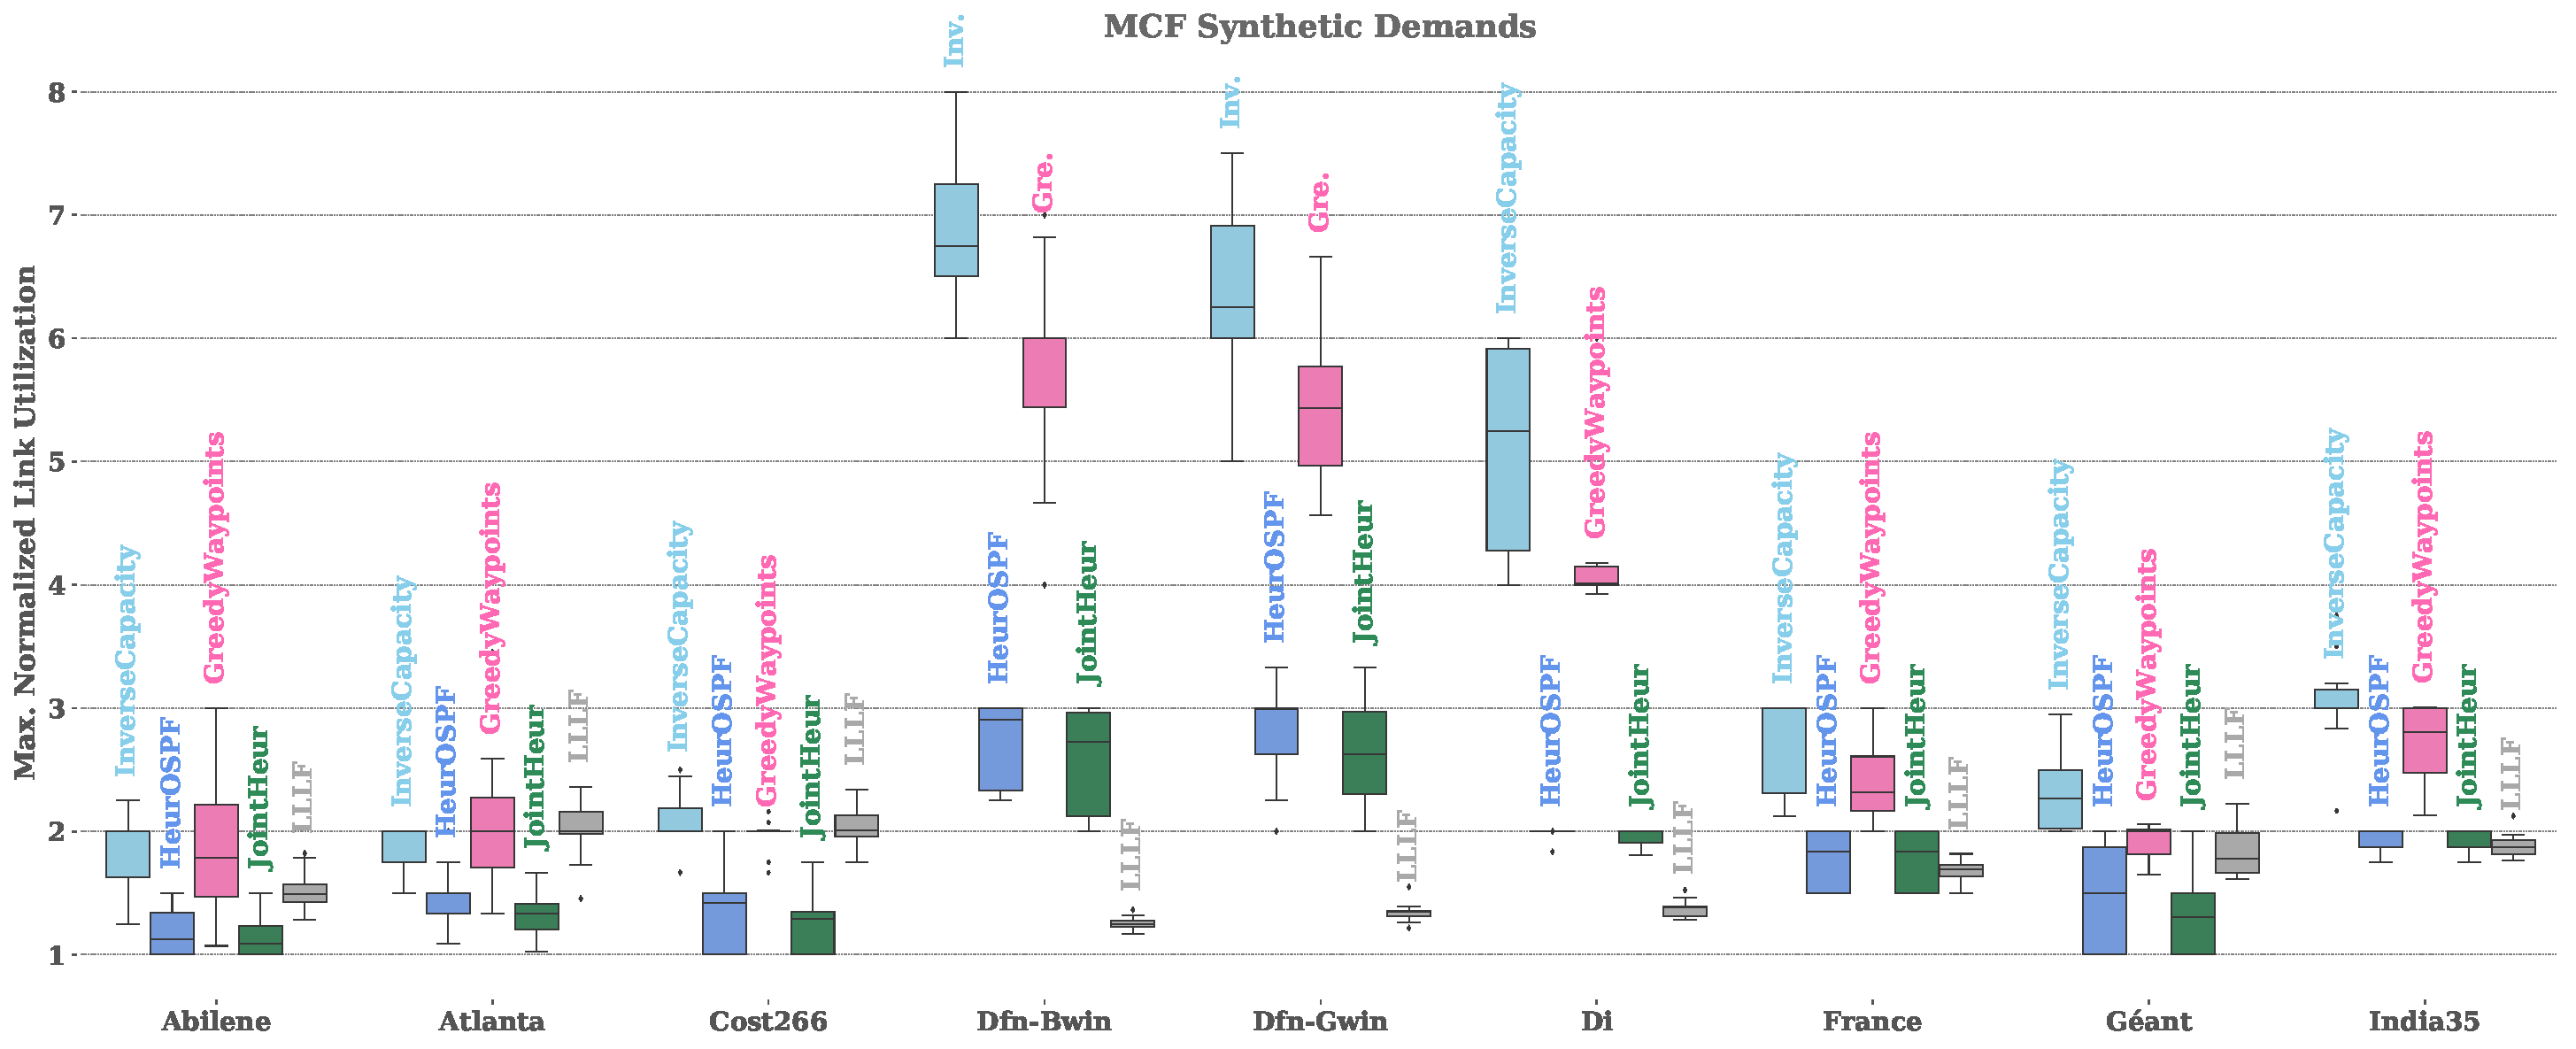
\includegraphics[width=\textwidth]{DA-Vorlage/bilder/algorithmus1/projekt1/all_topologies_objective_0.pdf}
        \end{subfigure}
        \begin{subfigure}{1.0\textwidth}
            \centering
            \caption{Synthetische Demands Laufzeit}
            \label{fig:ergebnisse_lllf_projekt1_2}
            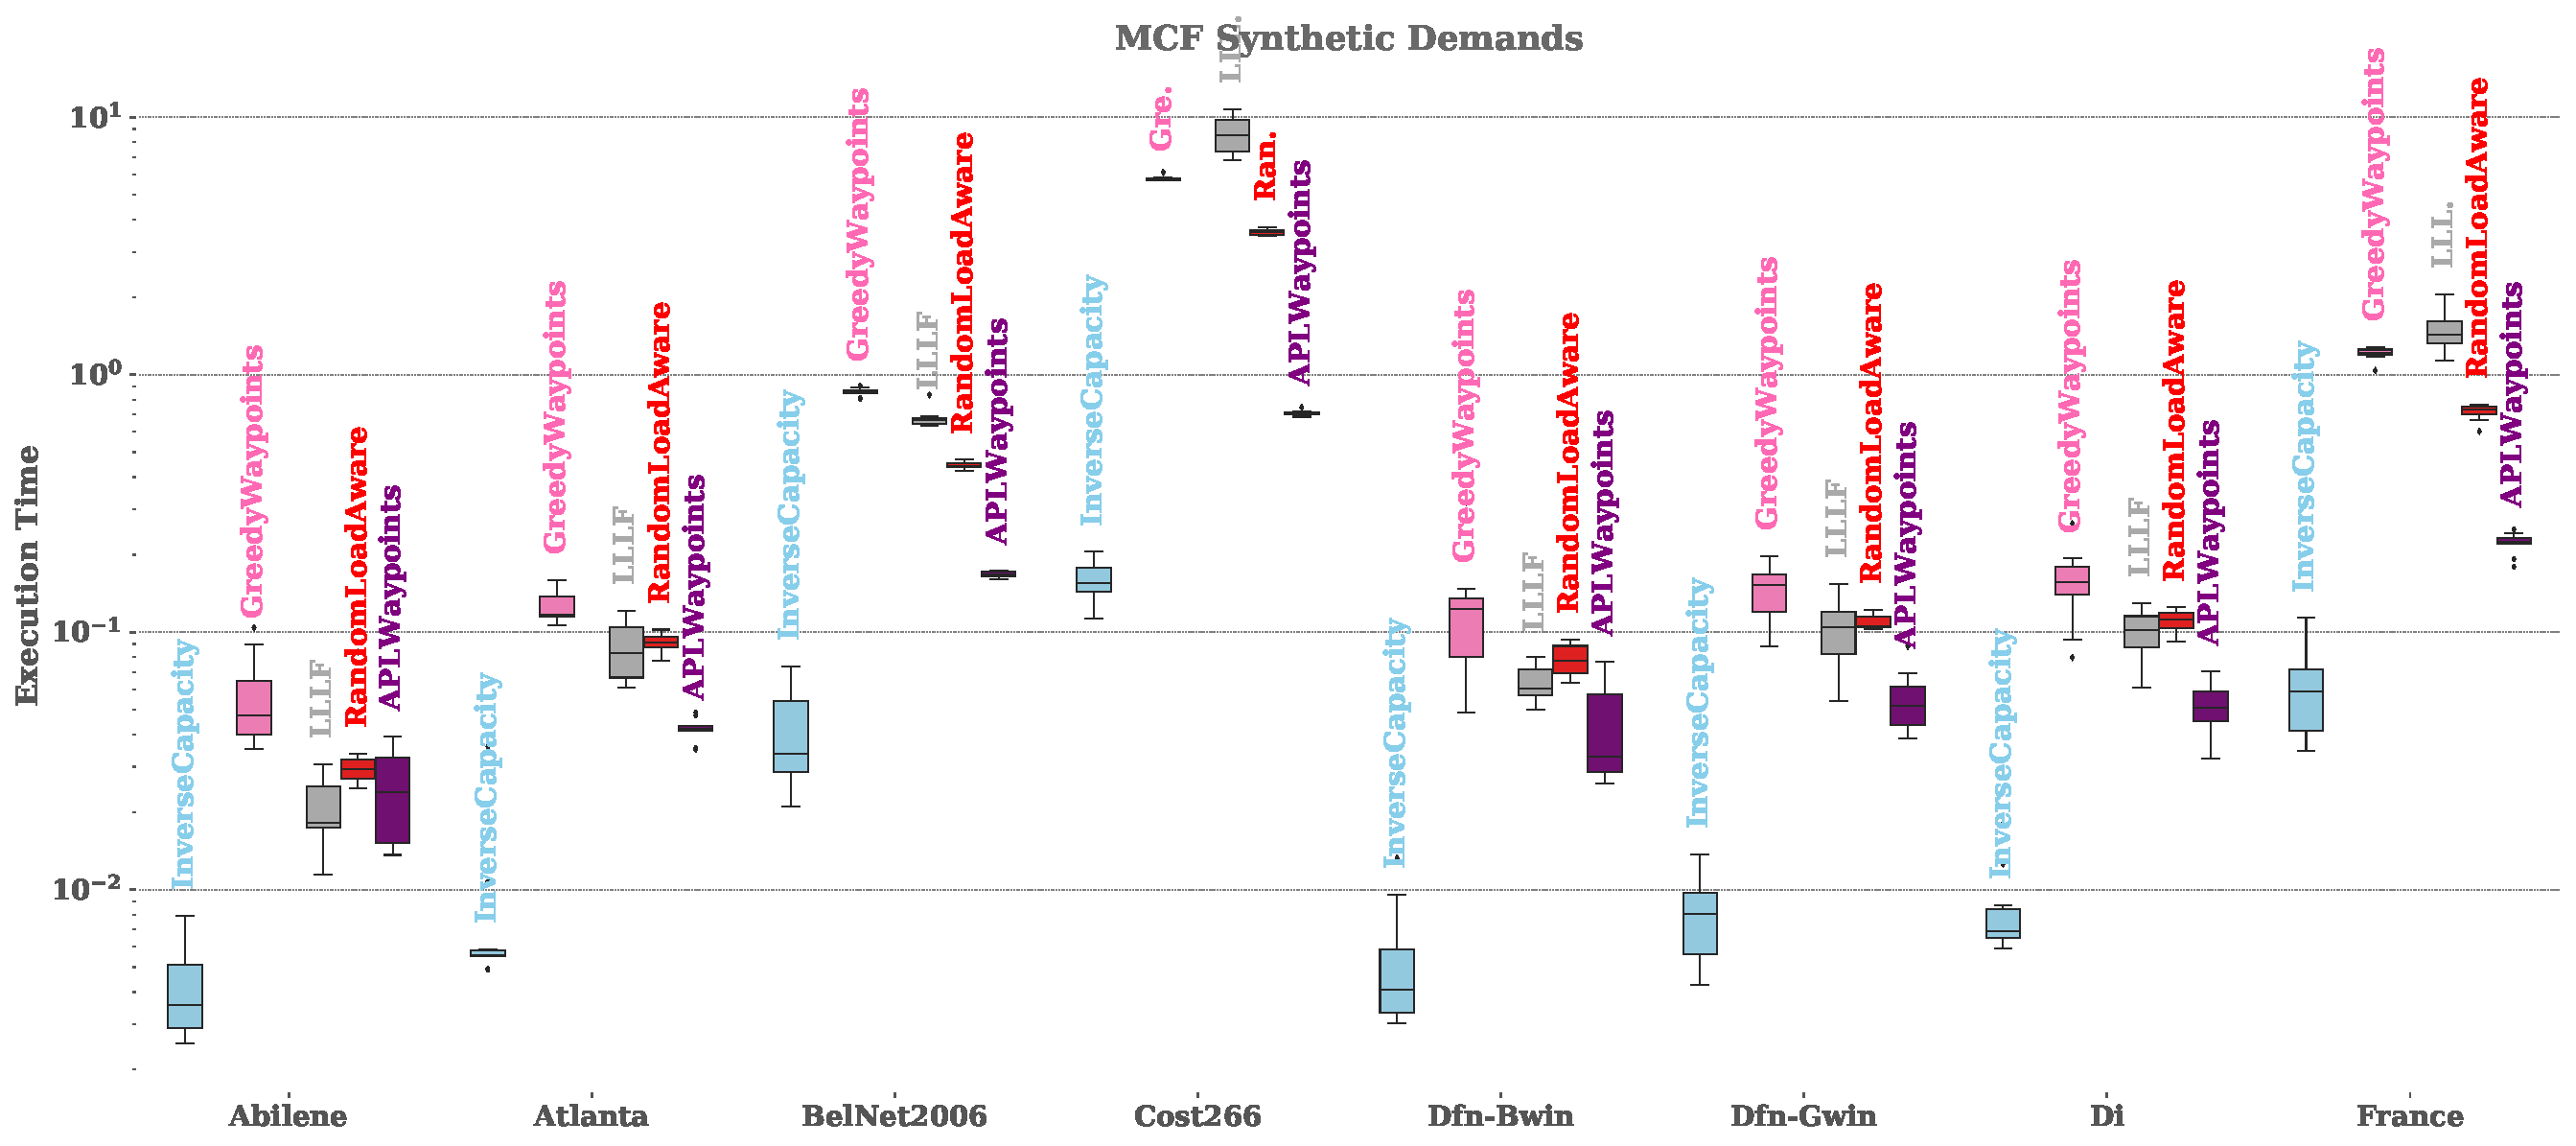
\includegraphics[width=\textwidth]{DA-Vorlage/bilder/algorithmus1/projekt1/all_topologies_execution_time_0.pdf}
        \end{subfigure}
        \begin{subfigure}{0.45\textwidth}
            \centering
            \caption{Echte Demands MLU}
            \label{fig:ergebnisse_lllf_projekt1_3}
            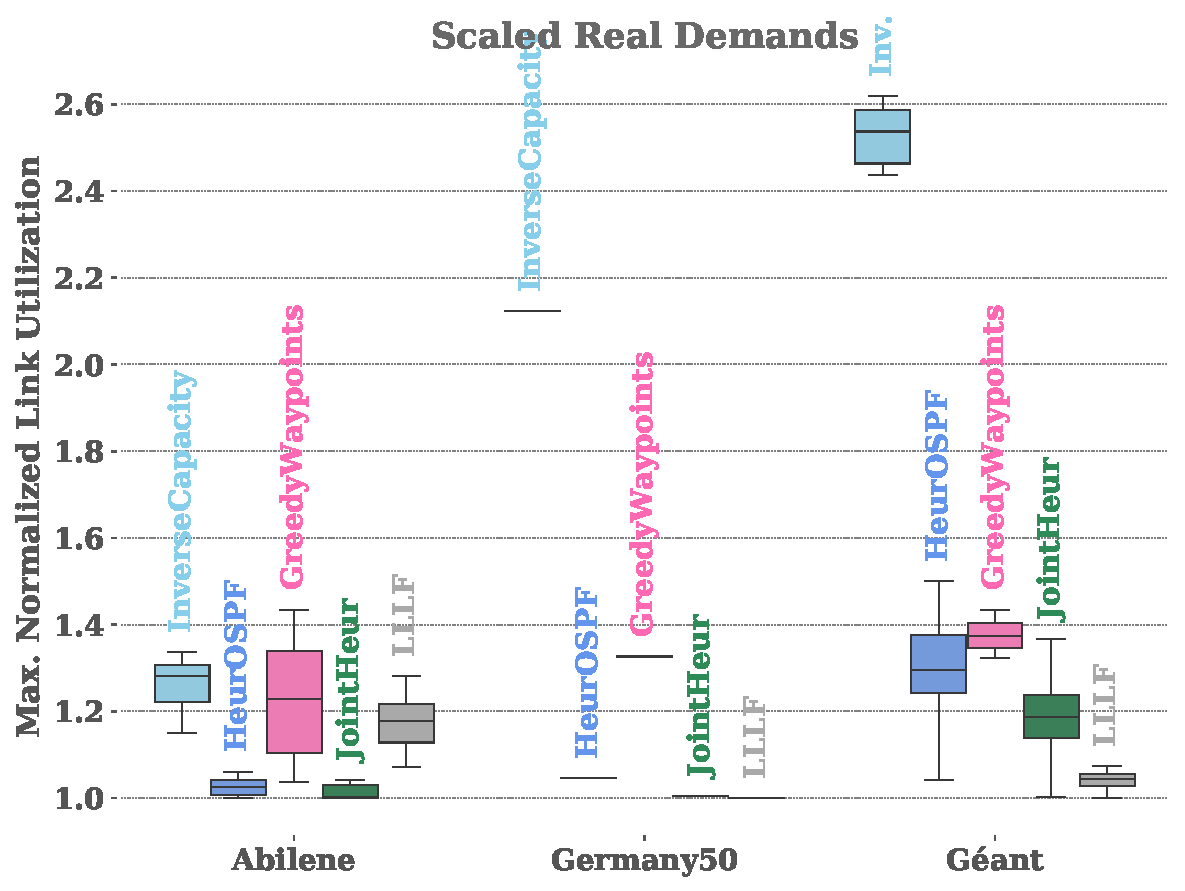
\includegraphics[width=\textwidth]{DA-Vorlage/bilder/algorithmus1/projekt1/real_demands_objective.pdf}
        \end{subfigure}
        \begin{subfigure}{0.45\textwidth}
            \centering
            \caption{Echte Demands Laufzeit}
            \label{fig:ergebnisse_lllf_projekt1_4}
            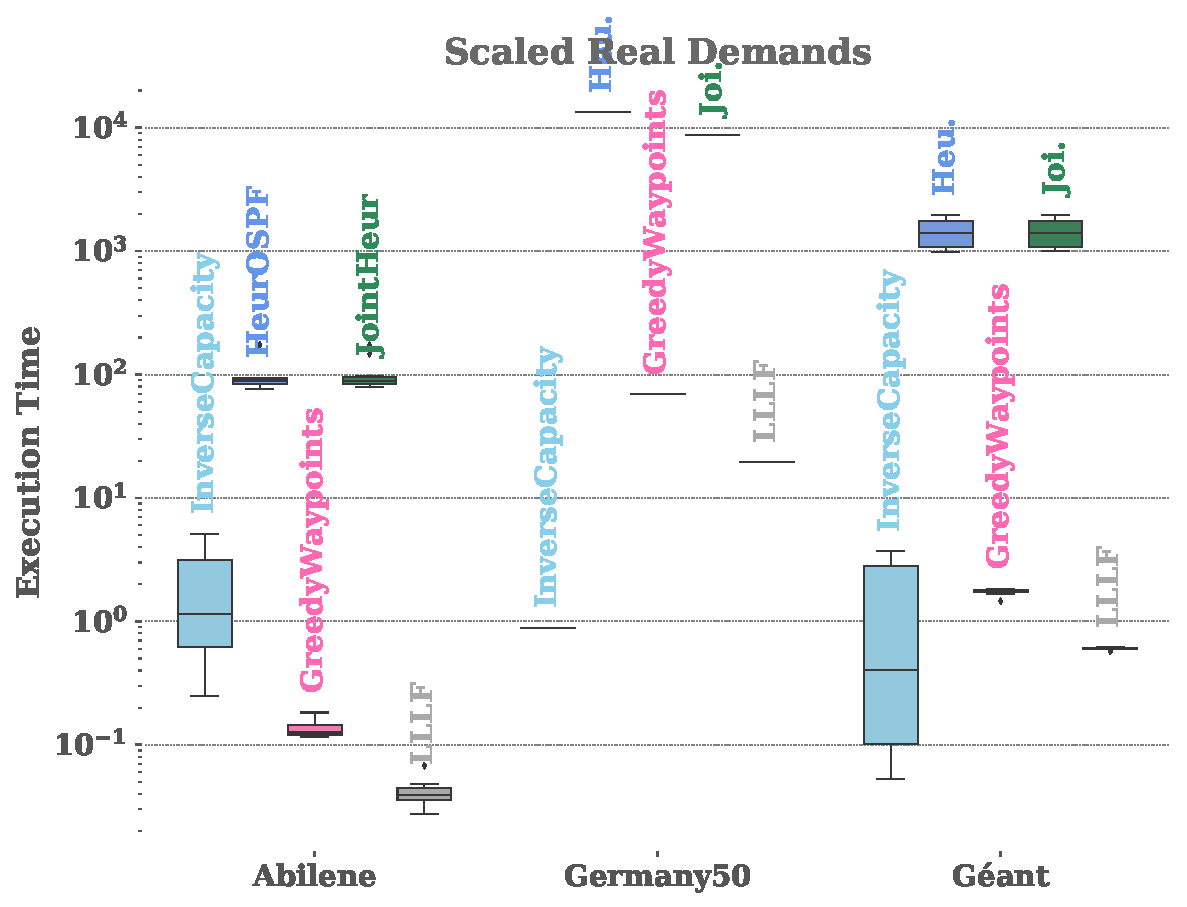
\includegraphics[width=\textwidth]{DA-Vorlage/bilder/algorithmus1/projekt1/real_demands_execution_time.pdf}
        \end{subfigure}
    \end{figure}

    In Projekt zwei wurden der Algorithmus dann auf einem eigenen Topologie simuliert. Da in Projekt 1 schon festgestellt wurde, dass der Algorithmus gut auf dichten Topologien, also welche mit vielen Kanten, funktioniert, haben wir folgende eigene Topologie \ref{fig:lllf-topologie} erstellt, wobei alle Kanten Kapazität 2 haben.

    \begin{figure}
        \centering
        \caption{Ergebnisse LLLF Projekt 2}
        \label{fig:ergebnisse_lllf_projekt1}
        \begin{subfigure}[c]{0.4\textwidth}
            \centering
            \caption{LLLF-Topologie}
            \label{fig:lllf-topologie} 
            \scalebox{0.8}{
                \begin{tikzpicture}[
                    node distance=7mm,
                    <->
                    ]
                    \node[state]                    (0)     {$0$};
                    \node[state, above=of 0]        (1)     {$1$};
                    \node[state, above=of 1]        (2)     {$2$};
                    \node[state, above right=of 2]  (3)     {$3$};
                    \node[state, right=of 3]        (4)     {$4$};
                    \node[state, right=of 4]        (5)     {$5$};
                    \node[state, below right=of 5]  (6)     {$6$};
                    \node[state, below=of 6]        (7)     {$7$};
                    \node[state, below=of 7]        (8)     {$8$};
                    \node[state, below left=of 8]   (9)     {$9$};
                    \node[state, left=of 9]         (10)    {$10$};
            
                    \path (0) edge[left]            node{}       (1);
                    \path (0) edge[bend left, left] node{}       (2);
                    \path (0) edge[left]            node{}       (6);
                    \path (0) edge[left]            node{}       (7);
                    \path (0) edge[left]            node{}       (8);
                    \path (0) edge[left]            node{}       (9);
                    \path (0) edge[left]            node{}       (10);
                    \path (0) edge[left]            node{}       (10);
                    
                    \path (1) edge[left]            node{}       (2);
                    \path (1) edge[left]            node{}       (3);
                    \path (1) edge[left]            node{}       (4);
                    \path (1) edge[left]            node{}       (5);
                    \path (1) edge[left]            node{}       (7);
                    \path (1) edge[left]            node{}       (9);
                    \path (1) edge[left]            node{}       (10);
                    
                    \path (2) edge[left]            node{}       (4);
                    \path (2) edge[left]            node{}       (5);
                    \path (2) edge[left]            node{}       (7);
                    \path (2) edge[left]            node{}       (8);
                    \path (2) edge[left]            node{}       (9);
                    \path (2) edge[left]            node{}       (10);
                    
                    \path (3) edge[left]            node{}       (4);
                    \path (3) edge[bend left, left] node{}       (5);
                    \path (3) edge[left]            node{}       (6);
                    \path (3) edge[left]            node{}       (7);
                    \path (3) edge[left]            node{}       (8);
                    \path (3) edge[left]            node{}       (9);
                    \path (3) edge[left]            node{}       (10);
                    
                    \path (4) edge[left]            node{}       (5);
                    \path (4) edge[left]            node{}       (6);
                    \path (4) edge[left]            node{}       (7);
                    \path (4) edge[left]            node{}       (8);
                    
                    \path (5) edge[left]            node{}       (7);
                    \path (5) edge[left]            node{}       (9);
                    \path (5) edge[left]            node{}       (10);
                    
                    \path (6) edge[left]            node{}       (7);
                    \path (6) edge[bend left, left] node{}       (8);
                    \path (6) edge[left]            node{}       (9);
                    \path (6) edge[left]            node{}       (10);
                    
                    \path (7) edge[left]            node{}       (9);
                    \path (7) edge[left]            node{}       (10);
                    
                    \path (8) edge[left]            node{}       (9);
                    \path (8) edge[left]            node{}       (10);
                \end{tikzpicture}
            }
        \end{subfigure}
        \begin{subfigure}[c]{0.55\textwidth}
            \centering
            \caption{Ergebnisse LLLF Projekt 2}
            \label{fig:ergebnisse_lllf_projekt2}
            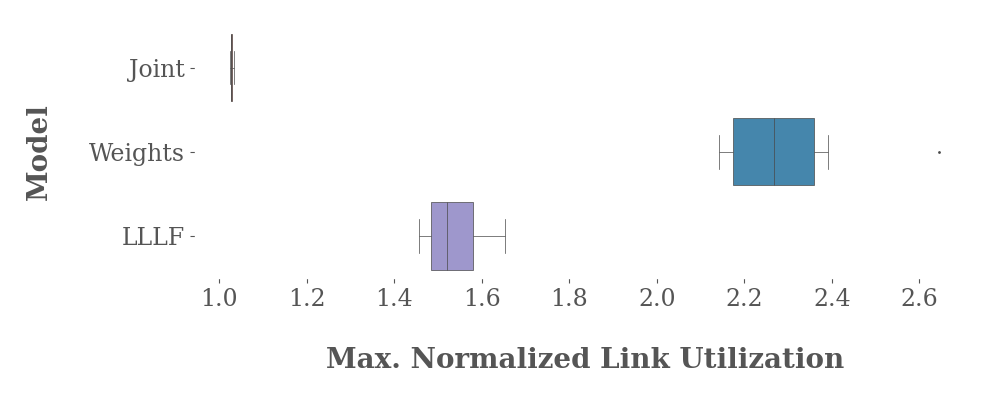
\includegraphics[width=\textwidth]{DA-Vorlage/bilder/algorithmus1/projekt2/result_lllf.png}
        \end{subfigure}
    \end{figure}

    Die benutzen Demands lauten wie folgt: 
    \begin{itemize}
        \item $s=8$, $t=1$, $d=1.0$ \qquad $s=8$, $t=1$, $d=1.0$ 
        \item $s=8$, $t=1$, $d=1.0$ \qquad $s=8$, $t=1$, $d=1.0$ 
        \item $s=8$, $t=1$, $d=1.0$ \qquad $s=6$, $t=4$, $d=1.0$ 
        \item $s=6$, $t=4$, $d=1.0$ \qquad $s=6$, $t=4$, $d=1.0$ 
        \item $s=6$, $t=4$, $d=1.0$ \qquad $s=6$, $t=4$, $d=1.0$ 
    \end{itemize}
    Die theoretische MLU die erreicht werden müsste wäre $0.5$. \\
    Man sieht in der Abbildung \ref{fig:ergebnisse_lllf_projekt2}, dass die theoretische MLU leider nicht erreicht wurde. Mögliche Probleme, die bei dazu geführt haben könnten, wären:
    \begin{itemize}
        \large
        \item Die ersten paar Tests waren fehlerhaft: 
        \begin{itemize}
            \item nuttcp-t: v6.1.2: Error: connect: Connection refused
            \item nuttcp-r: v6.1.2: Error: bind: Address already in use
        \end{itemize}
        \item Auch könnte es Probleme bei mehreren Demands mit selben Start und Ziel geben.
        \item Möglicherweise war die Topologie auch zu komplex für die Simulation.
    \end{itemize}

\section{Mögliche Verbesserungen und Ausblick}
    Um den Algorithmus noch besser zu machen, gibt es noch mögliche Verbesserungen, welche für die Ergebnisse aus den Projekten 1 und 2 teilweise schon implementiert wurden. Die erste Idee war, die Demands vorher zu sortieren, um die großen Demands auf die Topologie zu verteilen und danach mit kleinen aufzufüllen. Die zweite Idee war, bei mehreren besten Pfaden (geringste MLU), erst den kürzesten Pfad zu betrachten. Dadurch wird zu Topologie nicht unnötig belastet. Als dritte Idee, haben wir den Algorithmus nach initialer Verteilung der Demands auf Pfade mehrmals wiederholt ausgeführt, wobei bei jedem Durchlauf für jeden Demand geschaut wurde, ob ein neuer optimaler Pfad existiert. \\

    Abschließend kann man sagen, dass der LLLF-Algorithmus eine positive Bilanz hatte und sich gut in den schon existierenden Algorithmen angeschlossen hat. Der Algorithmus ist ein Beispiel dafür, wie klassische Graphenalgorithmen (hier: Dijkstra) anwendungsorientiert modifiziert werden können, um Lastverteilungen in Netzwerken effizient zu steuern. Trotz seiner heuristischen Natur stellt er in vielen praxisnahen Szenarien eine effektive Methode dar, um Netzwerkengpässe zu vermeiden und die Ressourcenauslastung zu balancieren.
